\documentclass[a4paper,12pt]{article}

% \usepackage[french]{babel}


\usepackage[utf8]{inputenc}
\usepackage[T1]{fontenc}
\usepackage{amssymb,amsthm,amsmath,amsfonts}
\usepackage{textcomp}
%\usepackage{bbm}
\usepackage{graphicx}

\usepackage{framed}

\def\BF{\begin{framed} }
\def\EF{\end{framed} }

\frenchspacing

\long\def\/*#1*/{}

\def\gal{\text{Gal}}

\setlength{\textwidth}{15cm}
\setlength{\hoffset}{0.46cm}
\setlength{\oddsidemargin}{0cm}
\setlength{\marginparsep}{0cm}
\setlength{\marginparwidth}{0cm}
\setlength{\textheight}{24.2cm}
\setlength{\headheight}{0cm}
\setlength{\topmargin}{0cm}
\setlength{\headsep}{0cm}
\setlength{\paperwidth}{29cm}

\def\RR{\mathbb{R}}
\def\CC{\mathbb{C}}
\def\NN{\mathbb{N}}
\def\ZZ{\mathbb{Z}}
\def\Q{\mathbb{Q}}
\def\F{\mathbb{F}}
\def\1{\mathbbm{1}}

% Usual sets of numbers  
\def\bA{{\Bbb A}}
\def\bC{{\Bbb C}}
\def\bF{{\Bbb F}}
\def\bK{{\Bbb K}}
\def\bN{{\Bbb N}}
\def\bP{{\Bbb P}}
\def\bQ{{\Bbb Q}}
\def\bR{{\Bbb R}}
\def\bZ{{\Bbb Z}}


\DeclareMathOperator{\pgcd}{pgcd}
\DeclareMathOperator{\ppcm}{ppcm}
\DeclareMathOperator{\GL}{GL}
\DeclareMathOperator{\Aut}{Aut}
\DeclareMathOperator{\Inn}{Inn}
\DeclareMathOperator{\id}{id}
\DeclareMathOperator{\End}{End}
\DeclareMathOperator{\Hom}{Hom}

\newcommand{\FF}{\mathbb{F}_q}

\def\ggauche{\textgravedbl}
\def\gdroite{\textacutedbl}


% Usual sets of numbers  
\def\bA{{\Bbb A}}
\def\bC{{\Bbb C}}
%\def{\bF{\Bbb F}}
\def\bK{{\Bbb K}}
\def\bN{{\Bbb N}}
\def\bP{{\Bbb P}}
\def\bQ{{\Bbb Q}}
\def\bR{{\Bbb R}}
\def\bZ{{\Bbb Z}}

\def\gc{\hbox{\goth c}}
\def\sevengc{\hbox{\sevengoth c}}
\def\mathfrak{\hbox{\goth S}}
\def\tr{\mathop{\rm tr}}
\def\Gal{\mathop{\rm Gal}}
\def\syquad#1#2{\left({#1\over #2}\right)}


\reversemarginpar

\newcommand{\dual}{\vee}

\newtheorem{enonce}{Exercice}
\newenvironment{E}[0]{\begin{enonce}\rm}{\bigskip \end{enonce}}

\begin{document}

Calculer la longueur de l'arc de la courbes paramétrées suivante :

\begin{enumerate}
\item
Une trochoïde est une courbe obtenue en traçant le mouvement décrit
par un point lié à un disque roulant sans glisser sur une droite.

  \begin{figure}[hb]
\centering
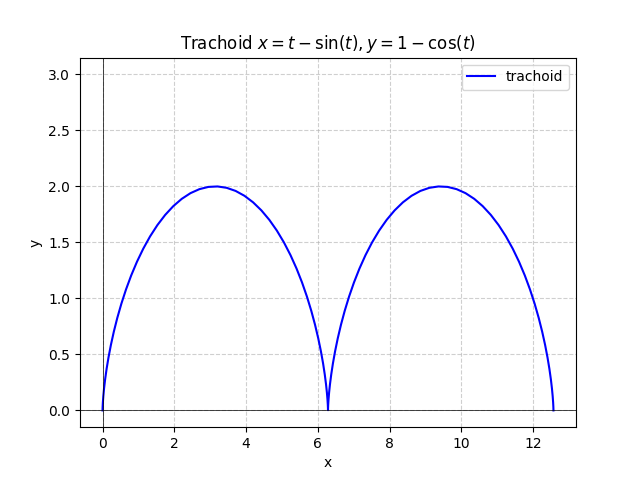
\includegraphics[scale=.5]{trachoid.png} 
  \label{pt graphic}
\end{figure}

% Calculer la longueur de l'arc de la courbe paramétrée suivante sur
% l'intervalle $[0,2\pi]$ :
% $$ x= \cos(t), y = \frac12 \sin(2t)$$
L'équation paramétrique d'une trochoïde est donnée par :

$$x=r\theta - d\sin(\theta),y=r - d\cos(\theta), \theta \in [0,2\pi]$$
où $r$ est le rayon du cercle, $d$ est la distance entre le point et le centre du cercle, et $\theta$ est l'angle de rotation du cercle.

\item
Une astroïde est une courbe plane, qui peut se définir de plusieurs
façons. En particulier, il est possible de l'obtenir en faisant
rouler un cercle de rayon $r = \frac14$ à l'intérieur d'un cercle de rayon 1. Pour cette raison, l'astroïde est une hypocycloïde de cercle à quatre points de rebroussement.

  \begin{figure}[hb]
\centering
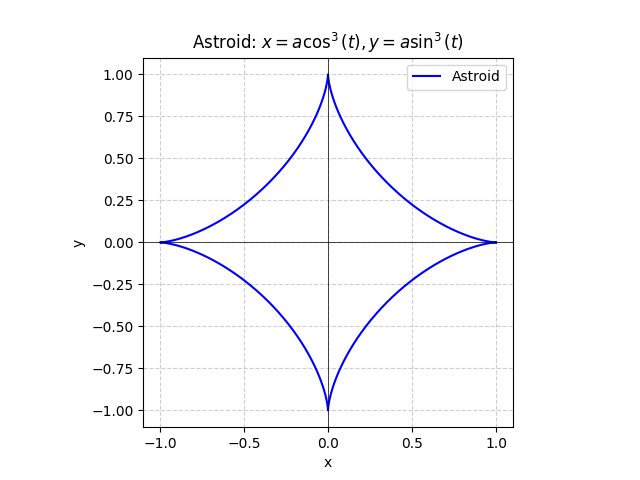
\includegraphics[scale=.7]{./asteroid.png} 
  \label{pt graphic}
\end{figure}
L'equation paramétrique de l'astroïde est donnée par :
$$ x= a\cos^3(t), y = a\sin^3(t)$$
où $a>0$ est une constante
et  $t\in[0,2\pi]$. Calculer la longueur de l'arc de cette courbe.
\item
Une lemniscate est une courbe plane ayant la forme d'un 8. Elle possède deux axes de symétrie perpendiculaires. Ceux-ci se coupent en un point double de la courbe, également son centre de symétrie.

  \begin{figure}[hb]
\centering
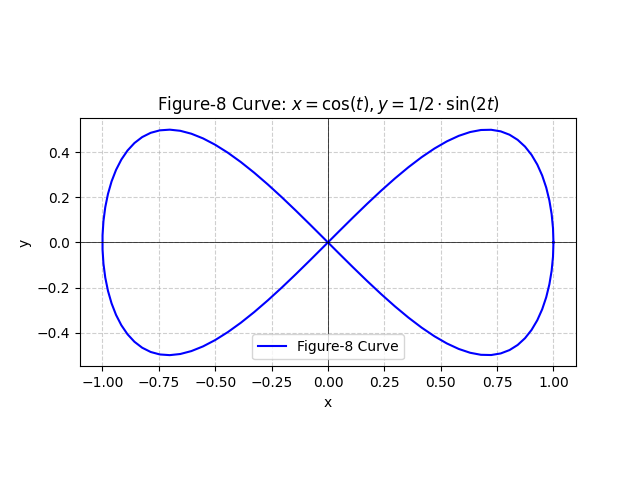
\includegraphics[scale=.7]{./fig8.png} 
  \label{pt graphic}
\end{figure}
Calculer la longueur de l'arc de la courbe paramétrée suivante sur
l'intervalle $[0,2\pi]$ :
$$ x= \cos(t), y = \frac12 \sin(2t)$$


Si on remplace $\frac12$ par $a$, on obtient une lemniscate,
ppeut-on calculer la longueur de l'arc de cette courbe paramétrée
sur l'intervalle $[0,2\pi]$ ?


\item

% ### 1. **Epicycloid** (Rolling Circle on the Outside of Another Circle)  
%    **Parametric Equations:**  
%    \[
%    x = (R + r) \cos\theta - r \cos\left(\frac{R + r}{r} \theta\right)
%    \]
%    \[
%    y = (R + r) \sin\theta - r \sin\left(\frac{R + r}{r} \theta\right)
%    \]


Hypocycloide ( Cercle roulant à l'intérieur d'un autre cercle)

Equation paramétrique:
   \[
   x = (R - r) \cos\theta + r \cos\left(\frac{R - r}{r} \theta\right)
   \]
   \[
   y = (R - r) \sin\theta - r \sin\left(\frac{R - r}{r}
   \theta\right), \quad \theta \in [0, 2\pi]
   \]

   où \( R \) est le rayon du cercle fixe, \( r \) est le rayon
   du cercle roulant, et \( \theta \) est l'angle de rotation du
   cercle roulant.


   Calculer la longueur de l'arc de la courbe paramétrée pour
   $R=1$ et $r= \frac12, \frac{1}{4}$.

  \begin{figure}[hb]
\centering
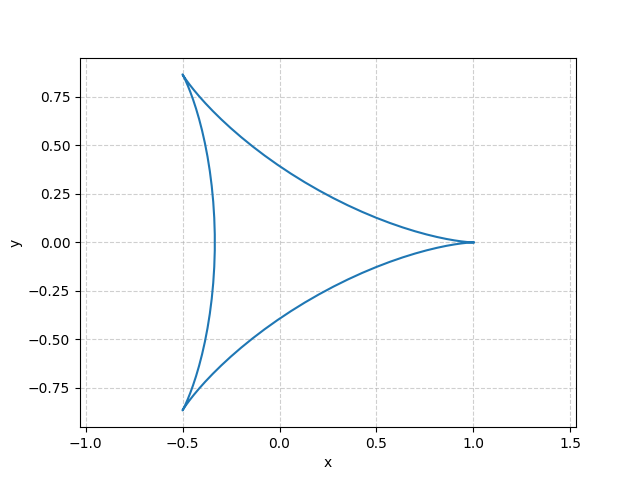
\includegraphics[scale=.8]{./hypocycloid.png} 
  \label{pt graphic}
\end{figure}

   % **Parametric Equations (Fresnel Integrals):**  
   % \[
   % x = \int_0^s \cos(t^2) \, dt, \quad y = \int_0^s \sin(t^2) \, dt
   % \]
   % The arc length is simply the parameter \( s \), making it a **natural curve for designing smooth transitions**, like in highways and railways.

---


\end{document}
